\chapter{Bangun Ruang dan Volume}\label{ch:g9:solids}

Geometri ruang bermula dengan keluarga kecil \omterm{def:g5:solids:def}{bangun ruang} --- \omterm{def:g7:areas:prism}{prisma},
\omterm{def:g7:areas:prism}{tabung}, \omterm{def:g8:solids:def}{limas}, \omterm{def:g8:solids:def}{kerucut}, bola --- dan dua pertanyaan: berapa banyak yang
dimuatnya (\omterm{def:g6:measure:volume}{volume}), dan apa yang kamu lihat ketika mengirisnya
(\omterm{prop:g9:solids:sections}{penampang})? Bab ini ditutup dengan kenyataan yang sangat penting
secara praktis: menskalakan \omterm{def:g5:solids:def}{bangun ruang} dengan $k$ mengalikan
\omterm{def:g6:measure:volume}{volumenya} dengan $k^3$.

\section{Bangun ruang klasik dan volumenya}

\begin{theorem}[Rumus volume]\label{thm:g9:solids:volumes}
Tulislah $B$ untuk luas alasnya dan $h$ untuk tingginya (yaitu jarak
antara alasnya dan sisi atau puncak yang di seberangnya).
\begin{center}
\renewcommand{\arraystretch}{1.5}
\begin{tabular}{l|l}
\omterm{def:g5:solids:def}{bangun ruang} & \omterm{def:g6:measure:volume}{volume} \\
\hline
\omterm{def:g7:areas:prism}{prisma}, \omterm{def:g7:areas:prism}{tabung} & $V = B \times h$ \\[5pt]
\omterm{def:g8:solids:def}{limas}, \omterm{def:g8:solids:def}{kerucut} & $V = \dfrac13\, B \times h$ \\[5pt]
bola berjari-jari $r$ & $V = \dfrac43\,\pi r^3$ \\
\end{tabular}
\end{center}
Untuk \omterm{def:g7:areas:prism}{tabung} dan \omterm{def:g8:solids:def}{kerucut} berjari-jari $r$, luas alasnya
$B = \pi r^2$; luas permukaan bolanya adalah $4\pi r^2$.
\end{theorem}
\admitted

\begin{omfigure}
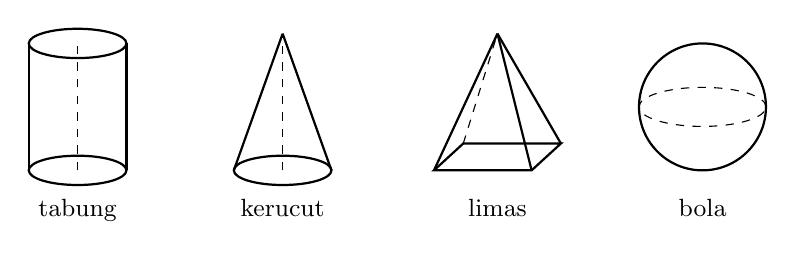
\begin{tikzpicture}[scale=0.62]
  % tabung
  \draw[thick] (0,0) ellipse (1 and 0.3);
  \draw[thick] (-1,0) -- (-1,2.6);
  \draw[thick] (1,0) -- (1,2.6);
  \draw[thick] (0,2.6) ellipse (1 and 0.3);
  \draw[dashed] (0,0) -- (0,2.6);
  \node[below, font=\small] at (0,-0.4) {tabung};
  % kerucut
  \begin{scope}[xshift=4.2cm]
  \draw[thick] (0,0) ellipse (1 and 0.3);
  \draw[thick] (-1,0) -- (0,2.8);
  \draw[thick] (1,0) -- (0,2.8);
  \draw[dashed] (0,0) -- (0,2.8);
  \node[below, font=\small] at (0,-0.4) {kerucut};
  \end{scope}
  % limas
  \begin{scope}[xshift=8.4cm]
  \draw[thick] (-1.1,0) -- (0.9,0) -- (1.5,0.55) -- (-0.5,0.55) -- cycle;
  \draw[thick] (-1.1,0) -- (0.2,2.8);
  \draw[thick] (0.9,0) -- (0.2,2.8);
  \draw[thick] (1.5,0.55) -- (0.2,2.8);
  \draw[dashed] (-0.5,0.55) -- (0.2,2.8);
  \node[below, font=\small] at (0.2,-0.4) {limas};
  \end{scope}
  % bola
  \begin{scope}[xshift=12.8cm]
  \draw[thick] (0,1.3) circle (1.3);
  \draw[dashed] (0,1.3) ellipse (1.3 and 0.4);
  \node[below, font=\small] at (0,-0.4) {bola};
  \end{scope}
\end{tikzpicture}

{\small \omterm{def:g5:solids:def}{Bangun ruang} bab ini. Untuk masing-masingnya, \omterm{def:g6:measure:volume}{volumenya} memuat
luas alas dan tinggi --- kecuali bolanya, yang hanya perlu \omterm{def:g3:shapes:shapes}{jari-jarinya}.}
\end{omfigure}

\begin{example}\label{ex:g9:solids:volumes}
Sebuah kaleng berbentuk \omterm{def:g7:areas:prism}{tabung} punya \omterm{def:g3:shapes:shapes}{jari-jari} $4$ cm dan tinggi $10$ cm:
\[
V = \pi r^2 h = \pi \times 16 \times 10 = 160\pi \approx 503 \text{ cm}^3
\approx 0.5 \text{ L}.
\]
\omterm{def:g8:solids:def}{Kerucut} dengan alas dan tinggi yang sama memuat sepertiganya:
$\frac{160\pi}{3} \approx 168$ cm$^3$. Bola berjari-jari $4$ cm:
$V = \frac43 \pi \times 64 = \frac{256\pi}{3} \approx 268$ cm$^3$.
\end{example}

\begin{example}[Sebuah limas selangkah demi selangkah]\label{ex:g9:solids:pyramid}
Sebuah \omterm{def:g8:solids:def}{limas} punya alas persegi bersisi $6$ m dan tinggi $5$ m.
\begin{enumerate}
  \item Luas alasnya: $B = 6^2 = 36$ m$^2$.
  \item \omterm{def:g6:measure:volume}{Volumenya}: $V = \frac13 \times 36 \times 5 = 60$ m$^3$.
\end{enumerate}
Perhatikan satuannya: kalau sisinya diberikan dalam cm dan tingginya
dalam m, salah satunya harus diubah lebih dahulu.
\end{example}

\section{Penampang oleh bidang}

\begin{proposition}[Penampang bangun ruang klasiknya]\label{prop:g9:solids:sections}
Memotong sebuah \omterm{def:g5:solids:def}{bangun ruang} dengan sebuah bidang menghasilkan bangun
datar, yaitu \emph{penampangnya}\index{penampang}:
\begin{itemize}
  \item \omterm{def:g7:areas:prism}{prisma} atau \omterm{def:g7:areas:prism}{tabung} yang dipotong \emph{\omterm{def:g6:lines:perp}{sejajar} dengan alasnya}
        memberi salinan alasnya, pada tiap ketinggian;
  \item \omterm{def:g8:solids:def}{limas} atau \omterm{def:g8:solids:def}{kerucut} yang dipotong \omterm{def:g6:lines:perp}{sejajar} dengan alasnya memberi
        \emph{pengecilan} alasnya: pada jarak $d$ dari puncaknya,
        \omterm{def:g9:thales:scaling}{faktor skalanya} adalah $k = \frac{d}{h}$;
  \item bola berjari-jari $r$ yang dipotong sebuah bidang pada jarak
        $d < r$ dari pusatnya memberi lingkaran berjari-jari
        $\sqrt{r^2 - d^2}$ (menurut teorema Pythagoras).
\end{itemize}
\end{proposition}
\admitted

\begin{omfigure}
\begin{tikzpicture}[scale=0.75]
  % kerucut dengan penampangnya
  \draw[thick] (0,0) ellipse (1.5 and 0.45);
  \draw[thick] (-1.5,0) -- (0,4.0);
  \draw[thick] (1.5,0) -- (0,4.0);
  \draw[omThm, thick, fill=omThm!12] (0,2.4) ellipse (0.6 and 0.18);
  \draw[dashed] (0,0) -- (0,4.0);
  \node[right, font=\small] at (0.1,4.0) {puncak};
  \draw[Stealth-Stealth, thin] (2.1,0) -- (2.1,4.0);
  \node[right, font=\small] at (2.1,2.0) {$h$};
  \draw[Stealth-Stealth, thin, omThm] (0.9,2.4) -- (0.9,4.0);
  \node[right, font=\small, omThm] at (0.92,3.2) {$d$};
  % bola dengan penampangnya
  \begin{scope}[xshift=7.6cm]
  \draw[thick] (0,2) circle (1.8);
  \draw[omThm, thick, fill=omThm!12] (0,2.9) ellipse (1.56 and 0.4);
  \fill (0,2) circle (1.5pt) node[below, font=\small] {$O$};
  \draw[thin] (0,2) -- (0,2.9) node[midway, left, font=\small] {$d$};
  \draw[thin] (0,2.9) -- (1.56,2.9)
    node[midway, above, font=\small] {$\sqrt{r^2 - d^2}$};
  \draw[thin] (0,2) -- (-1.27,0.72)
    node[midway, below right=-3pt, font=\small] {$r$};
  \end{scope}
\end{tikzpicture}

{\small Kiri: memotong \omterm{def:g8:solids:def}{kerucut} \omterm{def:g6:lines:perp}{sejajar} dengan alasnya pada jarak $d$
dari puncaknya memberi cakram yang terskala $k = \frac dh$. Kanan:
bidang yang berjarak $d$ dari pusat sebuah bola memotongnya menjadi
lingkaran berjari-jari $\sqrt{r^2 - d^2}$.}
\end{omfigure}

\begin{example}\label{ex:g9:solids:section}
Sebuah \omterm{def:g8:solids:def}{kerucut} punya \omterm{def:g3:shapes:shapes}{jari-jari} alas $6$ dan tinggi $9$. \omterm{prop:g9:solids:sections}{Penampang} oleh
bidang yang \omterm{def:g6:lines:perp}{sejajar} dengan alasnya, pada jarak $3$ dari puncaknya,
adalah cakram yang terskala $k = \frac39 = \frac13$: jadi \omterm{def:g3:shapes:shapes}{jari-jarinya}
$6 \times \frac13 = 2$.

Sebuah bola berjari-jari $5$ dipotong bidang pada jarak $3$ dari
pusatnya: \omterm{prop:g9:solids:sections}{penampangnya} lingkaran berjari-jari $\sqrt{25 - 9} = 4$.
\end{example}

\section{Menskalakan bangun ruang}

\begin{theorem}[Pengaruh penskalaan pada panjang, luas, volume]\label{thm:g9:solids:scaling}
Ketika sebuah \omterm{def:g5:solids:def}{bangun ruang} diperbesar atau dikecilkan dengan \omterm{def:g9:thales:scaling}{faktor
skala} $k > 0$:
\begin{itemize}
  \item semua panjangnya dikalikan $k$;
  \item semua luasnya dikalikan $k^2$;
  \item semua \omterm{def:g6:measure:volume}{volumenya} dikalikan $k^3$.
\end{itemize}
\end{theorem}
\admitted

\begin{example}\label{ex:g9:solids:scaling}
Sebuah mobil model berskala $\frac{1}{18}$: panjangnya adalah panjang
mobil yang sebenarnya dikalikan $k = \frac{1}{18}$, permukaan yang
dicatnya dikalikan $k^2 = \frac{1}{324}$, dan \omterm{def:g6:measure:volume}{volumenya} dikalikan
$k^3 = \frac{1}{5832}$.

Melipatduakan \omterm{def:g3:shapes:shapes}{jari-jari} sebuah bola ($k = 2$) mengalikan \omterm{def:g6:measure:volume}{volumenya}
dengan $2^3 = 8$: periksalah pada rumusnya,
$\frac43\pi (2r)^3 = \frac43 \pi \times 8r^3$.
\end{example}

\begin{example}[Kerucut terpancung]\label{ex:g9:solids:truncated}
Sebuah \omterm{def:g8:solids:def}{kerucut} setinggi $9$ dengan \omterm{def:g3:shapes:shapes}{jari-jari} alas $6$ (\omterm{def:g6:measure:volume}{volumenya}
$\frac13 \pi \times 36 \times 9 = 108\pi$) dipotong pada jarak $3$ dari
puncaknya, lalu \omterm{def:g8:solids:def}{kerucut} kecil di atas potongannya dibuang. \omterm{def:g8:solids:def}{Kerucut}
kecilnya adalah pengecilan dengan $k = \frac13$, jadi \omterm{def:g6:measure:volume}{volumenya}
$108\pi \times \left(\frac13\right)^3 = 4\pi$. \omterm{def:g5:solids:def}{Bangun ruang} yang
tersisa (yaitu \emph{\omterm{def:g8:solids:def}{kerucut} terpancung}) punya \omterm{def:g6:measure:volume}{volume}
$108\pi - 4\pi = 104\pi \approx 327$.
\end{example}

\section{Latihan}

\begin{exercise}[$\star$]\label{exo:g9:solids:1}
Hitunglah \omterm{def:g6:measure:volume}{volumenya}: sebuah \omterm{def:g5:solids:def}{balok} (\omterm{def:g7:areas:prism}{prisma} persegi panjang) berukuran
$4 \times 5 \times 12$; sebuah \omterm{def:g7:areas:prism}{tabung} berjari-jari $3$ dan tinggi $7$
(nilai persisnya dengan $\pi$, lalu \omterm{def:g4:numbers:round}{dibulatkan} ke satuan).
\end{exercise}

\begin{exercise}[$\star$]\label{exo:g9:solids:2}
Hitunglah \omterm{def:g6:measure:volume}{volume} \omterm{def:g8:solids:def}{kerucut} berjari-jari $5$ dan tinggi $12$, lalu \omterm{def:g6:measure:volume}{volume}
\omterm{def:g8:solids:def}{limas} dengan alas persegi panjang $8 \times 3$ dan tinggi $10$.
\end{exercise}

\begin{exercise}[$\star$]\label{exo:g9:solids:3}
Hitunglah \omterm{def:g6:measure:volume}{volume} dan luas permukaan bola berjari-jari $6$ (nilai
persisnya dengan $\pi$).
\end{exercise}

\begin{exercise}[$\star$]\label{exo:g9:solids:4}
Sebuah bola berjari-jari $10$ dipotong bidang pada jarak $8$ dari
pusatnya. Berapa \omterm{def:g3:shapes:shapes}{jari-jari} lingkaran \omterm{prop:g9:solids:sections}{penampangnya}?
\end{exercise}

\begin{exercise}[$\star\star$]\label{exo:g9:solids:5}
Sebuah \omterm{def:g8:solids:def}{kerucut} punya \omterm{def:g3:shapes:shapes}{jari-jari} alas $8$ dan tinggi $12$. Sebuah bidang
\omterm{def:g6:lines:perp}{sejajar} alasnya memotongnya pada jarak $9$ dari puncaknya. Hitunglah
\omterm{def:g3:shapes:shapes}{jari-jari} \omterm{prop:g9:solids:sections}{penampangnya}, lalu \omterm{def:g6:measure:volume}{volume} \omterm{def:g8:solids:def}{kerucut} kecil di atas potongannya.
\end{exercise}

\begin{exercise}[$\star\star$]\label{exo:g9:solids:6}
Sebuah gelas berbentuk \omterm{def:g7:areas:prism}{tabung} berjari-jari dalam $3$ cm berisi air
setinggi $10$ cm. Sebuah bola berjari-jari $2$ cm ditenggelamkan
seluruhnya di dalamnya. Naik berapa permukaan airnya? (\omterm{def:g6:measure:volume}{Volume} yang
ditambahkan menyebar pada luas alas gelasnya; berikan kenaikan
persisnya, lalu \omterm{def:g4:numbers:round}{bulatkan} ke milimeter.)
\end{exercise}

\begin{exercise}[$\star\star$]\label{exo:g9:solids:7}
Sebuah resep mengisi cetakan berbentuk bola berjari-jari $6$ cm. Kamu
hanya punya cetakan berbentuk bola berjari-jari $3$ cm. Berapa cetakan
kecil yang dapat kamu isi? (Jawablah tanpa menghitung salah satu
\omterm{def:g6:measure:volume}{volumenya} secara nyata.)
\end{exercise}

\begin{exercise}[$\star\star$]\label{exo:g9:solids:8}
Piramida Besar Giza punya alas persegi bersisi kira-kira $230$ m dan
tinggi kira-kira $147$ m. Taksirlah \omterm{def:g6:measure:volume}{volumenya}, lalu nyatakan dalam
jutaan meter kubik.
\end{exercise}

\begin{exercise}[$\star\star\star$]\label{exo:g9:solids:9}
Sebuah corong berbentuk \omterm{def:g8:solids:def}{kerucut} berjari-jari $6$ cm dan tinggi $12$ cm,
dengan puncaknya di bawah, diisi air sampai setengah \emph{tingginya}
(yang diukur dari puncaknya).
\begin{enumerate}
  \item Berapa bagian \omterm{def:g6:measure:volume}{volume} corongnya yang terisi?
  \item Kalau ia justru diisi dengan setengah \emph{\omterm{def:g6:measure:volume}{volumenya}} air,
        tunjukkan bahwa tinggi airnya $d$ memenuhi
        $\left(\frac{d}{12}\right)^3 = \frac12$, lalu berikan $d$
        sampai milimeter ($\sqrt[3]{0.5} \approx 0.7937$).
\end{enumerate}
\end{exercise}

\section{Soal: Batu nisan Archimedes}

\begin{problem}[{Soal akhir pekan --- bola itu dua pertiga tabungnya
(dua kali), tumpukan 1:2:3, dan hukum kuadrat--kubik yang melarang
adanya raksasa}]
\label{pb:g9:solids:1}
Archimedes membuktikan banyak teorema, tetapi satu teorema membuatnya
begitu bangga sehingga ia meminta \emph{gambarnya} dipahat pada
makamnya: sebuah bola yang bersarang di dalam \omterm{def:g7:areas:prism}{tabung} tersempitnya. Satu
abad kemudian penulis Romawi Cicero, yang menyisir semak berduri dekat
Syracusa, mengenali makam itu ``dari bolanya dan \omterm{def:g7:areas:prism}{tabungnya}''. Soal ini
mengambil kembali apa yang disandikan pahatan itu --- yaitu keajaiban
dua pertiga yang berganda --- lalu mengikuti \omterm{def:g6:measure:volume}{volume} dan permukaan
(\cref{thm:g9:solids:volumes},
\cref{thm:g9:solids:scaling}) menuju hukum yang mengatur raksasa, semut
dan planet yang mendingin.

\medskip
\noindent\textbf{Bagian I --- Pahatannya yang dipecahkan.}
Sebuah bola berjari-jari $r$ duduk persis di dalam sebuah \omterm{def:g7:areas:prism}{tabung}:
\omterm{def:g3:shapes:shapes}{jari-jarinya} sama, tingginya $2r$.
\begin{enumerate}
  \item Hitunglah \omterm{def:g6:measure:volume}{volume} \omterm{def:g7:areas:prism}{tabungnya} dalam $r$.
  \item Hitunglah perbandingan \omterm{def:g6:measure:volume}{volume} bolanya terhadap \omterm{def:g6:measure:volume}{volume}
        \omterm{def:g7:areas:prism}{tabungnya}. Mengapa Archimedes mungkin menyukai bahwa
        jawabannya tidak memuat $\pi$ dan tidak memuat $r$?
  \item Sekarang permukaannya: bandingkan luas permukaan bolanya
        dengan permukaan \emph{seluruh} \omterm{def:g7:areas:prism}{tabungnya} (bagian selimutnya
        ditambah kedua tutupnya). Perbandingan apa yang muncul ---
        sekali lagi?
  \item Ruang kosong antara bolanya dan \omterm{def:g7:areas:prism}{tabungnya} punya \omterm{def:g6:measure:volume}{volume}
        $2\pi r^3 - \frac43\pi r^3$. Tunjukkan bahwa sisa ini
        persis sama dengan \omterm{def:g6:measure:volume}{volume} \emph{dua \omterm{def:g8:solids:def}{kerucut}} berjari-jari
        $r$ dan tinggi $r$.
  \item Sebuah bola basket berjari-jari $12$ cm dijual dalam kotak
        berbentuk \omterm{def:g7:areas:prism}{tabung} yang tersempit. Hitunglah kedua \omterm{def:g6:measure:volume}{volumenya}
        (sampai $100$ cm$^3$ terdekat) dan berapa persen kotaknya
        yang kosong.
\end{enumerate}

\medskip
\noindent\textbf{Bagian II --- Mangkuk, cetakan dan bulan.}
\begin{enumerate}[resume]
  \item Sebuah mangkuk setengah bola berjari-jari $10$ cm. Hitunglah
        \omterm{def:g2:measure:units}{daya tampungnya}, dalam cm$^3$ dan dalam liter (sampai desiliter).
  \item Tumpukan 1:2:3: sebuah \omterm{def:g8:solids:def}{kerucut}, sebuah setengah bola dan
        sebuah \omterm{def:g7:areas:prism}{tabung}, semuanya berjari-jari $10$ cm dan tinggi
        $10$ cm. Hitunglah ketiga \omterm{def:g6:measure:volume}{volumenya} lalu periksalah
        perbandingan legendarisnya
        $1 : 2 : 3$. (Archimedes tentu menyukai yang ini juga.)
  \item Sebuah bola cokelat berjari-jari $3$ cm dilelehkan ke dalam
        cetakan berbentuk \omterm{def:g7:areas:prism}{tabung} berjari-jari $3$ cm. Tinggi berapa
        yang dicapai cokelatnya? (\omterm{def:g9:fractions:fraction}{Pecahan} yang persis, lalu sampai
        milimeter.)
  \item \omterm{def:g3:shapes:shapes}{Jari-jari} Bumi kira-kira $6\,371$ km, \omterm{def:g3:shapes:shapes}{jari-jari} Bulan
        kira-kira $1\,737$ km. Hitunglah perbandingan \omterm{def:g3:shapes:shapes}{jari-jarinya},
        lalu --- dengan \cref{thm:g9:solids:scaling} --- perbandingan
        \omterm{def:g6:measure:volume}{volumenya}: berapa Bulan yang akan muat ke dalam Bumi yang
        berongga, menurut \omterm{def:g6:measure:volume}{volumenya}?
  \item Dari teorema yang sama: berapa perbandingan
        \emph{luas permukaan} Bumi terhadap Bulan? Dan secara umum,
        ketika \omterm{def:g3:shapes:shapes}{jari-jari} sebuah balon berlipat dua, apa yang terjadi
        pada \omterm{def:g6:measure:volume}{volumenya} dan pada permukaannya? Nyatakan \emph{hukum
        kuadrat--kubiknya}: ketika sebuah bentuk membesar skalanya,
        \omterm{def:g6:measure:volume}{volumenya} melampaui permukaannya.
\end{enumerate}

\medskip
\noindent\textbf{Bagian III --- Hukum kuadrat--kubik menguasai
dunia.}
\begin{enumerate}[resume]
  \item Alasan Galileo terhadap raksasa: bayangkan seorang manusia
        yang diskalakan naik dengan faktor $10$, dengan perbandingan
        yang sama. Dengan faktor berapa beratnya tumbuh (berat
        mengikuti \omterm{def:g6:measure:volume}{volume})? Dengan faktor berapa \omterm{prop:g9:solids:sections}{penampang} tulangnya
        tumbuh (yaitu sebuah luas)? Lalu dengan faktor berapa
        \emph{tekanan} pada tiap sentimeter persegi tulangnya
        tumbuh --- dan apa yang terjadi pada raksasanya?
  \item Hukum yang sama secara terbalik menjelaskan kepahlawanan
        semut: kekuatan mengikuti \omterm{prop:g9:solids:sections}{penampang} otot (yaitu luas), berat
        mengikuti \omterm{def:g6:measure:volume}{volume}. Untuk hewan yang $100$ kali lebih kecil
        pada tiap arahnya, dengan faktor berapa berat dan kekuatannya
        mengerut, dan dengan faktor berapa perbandingan kekuatan
        terhadap beratnya membaik?
  \item Panas dihasilkan \omterm{def:g6:measure:volume}{volume} tubuhnya dan hilang lewat
        permukaannya. Tunjukkan bahwa untuk sebuah bola perbandingan
        permukaan terhadap \omterm{def:g6:measure:volume}{volumenya} adalah $\frac{3}{r}$, lalu
        hitunglah perbandingan itu untuk $r = 1$ dan $r = 2$. Mana
        yang lebih cepat mendingin, tikus atau beruang --- dan
        mengapa bayi perlu topi pada musim dingin?
  \item Dua jeruk berbentuk bola berjari-jari $4$ cm dan $5$ cm
        dijual dengan harga yang sama. Hitunglah perbandingan
        \omterm{def:g6:measure:volume}{volumenya}: berapa kali lebih banyak jeruk yang diberikan
        yang besar untuk uang yang sama?
  \item Penutupnya: uraikan dengan tepat apa yang disandikan gambar
        batu nisannya --- yaitu kedua ``dua pertiga'' pada pertanyaan
        2 dan 3 --- lalu jawablah Cicero dalam satu kalimat: mengapa
        seorang ahli matematika akan memilih, mengalahkan setiap
        penaklukan kejeniusan keteknikannya, sebuah bola di dalam
        \omterm{def:g7:areas:prism}{tabung}?

\end{enumerate}
\end{problem}
